\documentclass[]{article}
\usepackage{lmodern}
\usepackage{amssymb,amsmath}
\usepackage{ifxetex,ifluatex}
\usepackage{fixltx2e} % provides \textsubscript
\ifnum 0\ifxetex 1\fi\ifluatex 1\fi=0 % if pdftex
  \usepackage[T1]{fontenc}
  \usepackage[utf8]{inputenc}
\else % if luatex or xelatex
  \ifxetex
    \usepackage{mathspec}
  \else
    \usepackage{fontspec}
  \fi
  \defaultfontfeatures{Ligatures=TeX,Scale=MatchLowercase}
\fi
% use upquote if available, for straight quotes in verbatim environments
\IfFileExists{upquote.sty}{\usepackage{upquote}}{}
% use microtype if available
\IfFileExists{microtype.sty}{%
\usepackage{microtype}
\UseMicrotypeSet[protrusion]{basicmath} % disable protrusion for tt fonts
}{}
\usepackage[margin=1in]{geometry}
\usepackage{hyperref}
\hypersetup{unicode=true,
            pdftitle={Chapter 7 - Inference for Numerical Data},
            pdfauthor={Salma Elshahawy},
            pdfborder={0 0 0},
            breaklinks=true}
\urlstyle{same}  % don't use monospace font for urls
\usepackage{color}
\usepackage{fancyvrb}
\newcommand{\VerbBar}{|}
\newcommand{\VERB}{\Verb[commandchars=\\\{\}]}
\DefineVerbatimEnvironment{Highlighting}{Verbatim}{commandchars=\\\{\}}
% Add ',fontsize=\small' for more characters per line
\usepackage{framed}
\definecolor{shadecolor}{RGB}{248,248,248}
\newenvironment{Shaded}{\begin{snugshade}}{\end{snugshade}}
\newcommand{\AlertTok}[1]{\textcolor[rgb]{0.94,0.16,0.16}{#1}}
\newcommand{\AnnotationTok}[1]{\textcolor[rgb]{0.56,0.35,0.01}{\textbf{\textit{#1}}}}
\newcommand{\AttributeTok}[1]{\textcolor[rgb]{0.77,0.63,0.00}{#1}}
\newcommand{\BaseNTok}[1]{\textcolor[rgb]{0.00,0.00,0.81}{#1}}
\newcommand{\BuiltInTok}[1]{#1}
\newcommand{\CharTok}[1]{\textcolor[rgb]{0.31,0.60,0.02}{#1}}
\newcommand{\CommentTok}[1]{\textcolor[rgb]{0.56,0.35,0.01}{\textit{#1}}}
\newcommand{\CommentVarTok}[1]{\textcolor[rgb]{0.56,0.35,0.01}{\textbf{\textit{#1}}}}
\newcommand{\ConstantTok}[1]{\textcolor[rgb]{0.00,0.00,0.00}{#1}}
\newcommand{\ControlFlowTok}[1]{\textcolor[rgb]{0.13,0.29,0.53}{\textbf{#1}}}
\newcommand{\DataTypeTok}[1]{\textcolor[rgb]{0.13,0.29,0.53}{#1}}
\newcommand{\DecValTok}[1]{\textcolor[rgb]{0.00,0.00,0.81}{#1}}
\newcommand{\DocumentationTok}[1]{\textcolor[rgb]{0.56,0.35,0.01}{\textbf{\textit{#1}}}}
\newcommand{\ErrorTok}[1]{\textcolor[rgb]{0.64,0.00,0.00}{\textbf{#1}}}
\newcommand{\ExtensionTok}[1]{#1}
\newcommand{\FloatTok}[1]{\textcolor[rgb]{0.00,0.00,0.81}{#1}}
\newcommand{\FunctionTok}[1]{\textcolor[rgb]{0.00,0.00,0.00}{#1}}
\newcommand{\ImportTok}[1]{#1}
\newcommand{\InformationTok}[1]{\textcolor[rgb]{0.56,0.35,0.01}{\textbf{\textit{#1}}}}
\newcommand{\KeywordTok}[1]{\textcolor[rgb]{0.13,0.29,0.53}{\textbf{#1}}}
\newcommand{\NormalTok}[1]{#1}
\newcommand{\OperatorTok}[1]{\textcolor[rgb]{0.81,0.36,0.00}{\textbf{#1}}}
\newcommand{\OtherTok}[1]{\textcolor[rgb]{0.56,0.35,0.01}{#1}}
\newcommand{\PreprocessorTok}[1]{\textcolor[rgb]{0.56,0.35,0.01}{\textit{#1}}}
\newcommand{\RegionMarkerTok}[1]{#1}
\newcommand{\SpecialCharTok}[1]{\textcolor[rgb]{0.00,0.00,0.00}{#1}}
\newcommand{\SpecialStringTok}[1]{\textcolor[rgb]{0.31,0.60,0.02}{#1}}
\newcommand{\StringTok}[1]{\textcolor[rgb]{0.31,0.60,0.02}{#1}}
\newcommand{\VariableTok}[1]{\textcolor[rgb]{0.00,0.00,0.00}{#1}}
\newcommand{\VerbatimStringTok}[1]{\textcolor[rgb]{0.31,0.60,0.02}{#1}}
\newcommand{\WarningTok}[1]{\textcolor[rgb]{0.56,0.35,0.01}{\textbf{\textit{#1}}}}
\usepackage{graphicx,grffile}
\makeatletter
\def\maxwidth{\ifdim\Gin@nat@width>\linewidth\linewidth\else\Gin@nat@width\fi}
\def\maxheight{\ifdim\Gin@nat@height>\textheight\textheight\else\Gin@nat@height\fi}
\makeatother
% Scale images if necessary, so that they will not overflow the page
% margins by default, and it is still possible to overwrite the defaults
% using explicit options in \includegraphics[width, height, ...]{}
\setkeys{Gin}{width=\maxwidth,height=\maxheight,keepaspectratio}
\IfFileExists{parskip.sty}{%
\usepackage{parskip}
}{% else
\setlength{\parindent}{0pt}
\setlength{\parskip}{6pt plus 2pt minus 1pt}
}
\setlength{\emergencystretch}{3em}  % prevent overfull lines
\providecommand{\tightlist}{%
  \setlength{\itemsep}{0pt}\setlength{\parskip}{0pt}}
\setcounter{secnumdepth}{0}
% Redefines (sub)paragraphs to behave more like sections
\ifx\paragraph\undefined\else
\let\oldparagraph\paragraph
\renewcommand{\paragraph}[1]{\oldparagraph{#1}\mbox{}}
\fi
\ifx\subparagraph\undefined\else
\let\oldsubparagraph\subparagraph
\renewcommand{\subparagraph}[1]{\oldsubparagraph{#1}\mbox{}}
\fi

%%% Use protect on footnotes to avoid problems with footnotes in titles
\let\rmarkdownfootnote\footnote%
\def\footnote{\protect\rmarkdownfootnote}

%%% Change title format to be more compact
\usepackage{titling}

% Create subtitle command for use in maketitle
\providecommand{\subtitle}[1]{
  \posttitle{
    \begin{center}\large#1\end{center}
    }
}

\setlength{\droptitle}{-2em}

  \title{Chapter 7 - Inference for Numerical Data}
    \pretitle{\vspace{\droptitle}\centering\huge}
  \posttitle{\par}
    \author{Salma Elshahawy}
    \preauthor{\centering\large\emph}
  \postauthor{\par}
    \date{}
    \predate{}\postdate{}
  
\usepackage{geometry}
\usepackage{multicol}
\usepackage{multirow}
\usepackage{xcolor}

\begin{document}
\maketitle

\textbf{Working backwards, Part II.} (5.24, p.~203) A 90\% confidence
interval for a population mean is (65, 77). The population distribution
is approximately normal and the population standard deviation is
unknown. This confidence interval is based on a simple random sample of
25 observations. Calculate the sample mean, the margin of error, and the
sample standard deviation.

\begin{Shaded}
\begin{Highlighting}[]
\NormalTok{n <-}\StringTok{ }\DecValTok{25} \CommentTok{# the sample is below 30}
\NormalTok{df <-}\StringTok{ }\DecValTok{24}
\NormalTok{upper <-}\StringTok{ }\DecValTok{77}
\NormalTok{lower <-}\StringTok{ }\DecValTok{65}
\NormalTok{s_hat <-}\StringTok{ }\NormalTok{(}\DecValTok{77} \OperatorTok{+}\StringTok{ }\DecValTok{65}\NormalTok{) }\OperatorTok{/}\StringTok{ }\DecValTok{2}
\KeywordTok{paste0}\NormalTok{(}\StringTok{"Sample mean= "}\NormalTok{,s_hat) }\CommentTok{#sample mean}
\end{Highlighting}
\end{Shaded}

\begin{verbatim}
## [1] "Sample mean= 71"
\end{verbatim}

\begin{Shaded}
\begin{Highlighting}[]
\NormalTok{ME <-}\StringTok{ }\NormalTok{(}\DecValTok{77} \OperatorTok{-}\StringTok{ }\DecValTok{65}\NormalTok{) }\OperatorTok{/}\StringTok{ }\DecValTok{2}
\KeywordTok{paste0}\NormalTok{(}\StringTok{"Margin of error= "}\NormalTok{,ME) }\CommentTok{# margin of error}
\end{Highlighting}
\end{Shaded}

\begin{verbatim}
## [1] "Margin of error= 6"
\end{verbatim}

\begin{Shaded}
\begin{Highlighting}[]
\NormalTok{t <-}\StringTok{ }\FloatTok{1.711} \CommentTok{# two tails t-tables }
\NormalTok{SE_hat <-}\StringTok{ }\NormalTok{(upper }\OperatorTok{-}\StringTok{ }\NormalTok{s_hat) }\OperatorTok{/}\StringTok{ }\NormalTok{t}

\NormalTok{sd_hat <-}\StringTok{ }\NormalTok{SE_hat }\OperatorTok{*}\StringTok{ }\KeywordTok{sqrt}\NormalTok{(n)}
\KeywordTok{paste0}\NormalTok{(}\StringTok{"Sample standard deviation= "}\NormalTok{,sd_hat)}
\end{Highlighting}
\end{Shaded}

\begin{verbatim}
## [1] "Sample standard deviation= 17.5336060783168"
\end{verbatim}

\begin{center}\rule{0.5\linewidth}{\linethickness}\end{center}

\clearpage

\textbf{SAT scores.} (7.14, p.~261) SAT scores of students at an Ivy
League college are distributed with a standard deviation of 250 points.
Two statistics students, Raina and Luke, want to estimate the average
SAT score of students at this college as part of a class project. They
want their margin of error to be no more than 25 points.

\begin{enumerate}
\def\labelenumi{(\alph{enumi})}
\tightlist
\item
  Raina wants to use a 90\% confidence interval. How large a sample
  should she collect?
\item
  Luke wants to use a 99\% confidence interval. Without calculating the
  actual sample size, determine whether his sample should be larger or
  smaller than Raina's, and explain your reasoning.
\item
  Calculate the minimum required sample size for Luke.
\end{enumerate}

\begin{Shaded}
\begin{Highlighting}[]
\NormalTok{s_hat <-}\StringTok{ }\DecValTok{250} 
\NormalTok{ME <-}\StringTok{ }\DecValTok{25}
\NormalTok{z <-}\StringTok{ }\FloatTok{1.645} \CommentTok{# alpha is 0.1 because of 90% confidence interval from the table}
\NormalTok{n <-}\StringTok{ }\NormalTok{((z }\OperatorTok{*}\StringTok{ }\NormalTok{s_hat) }\OperatorTok{/}\StringTok{ }\NormalTok{ME) }\OperatorTok{^}\StringTok{ }\DecValTok{2}
\KeywordTok{paste0}\NormalTok{ (}\StringTok{"(a) Number of people needed for Raina sample is: "}\NormalTok{,}\KeywordTok{round}\NormalTok{(n, }\DataTypeTok{digits =} \DecValTok{0}\NormalTok{))}
\end{Highlighting}
\end{Shaded}

\begin{verbatim}
## [1] "(a) Number of people needed for Raina sample is: 271"
\end{verbatim}

\begin{enumerate}
\def\labelenumi{(\alph{enumi})}
\setcounter{enumi}{1}
\tightlist
\item
  Luke sampe size should be larger than Raina, because when we increase
  the confidence interval, the standard deviation increase,so as a
  result the number of samples should be bigger.
\end{enumerate}

\begin{Shaded}
\begin{Highlighting}[]
\NormalTok{s_hat <-}\StringTok{ }\DecValTok{250} 
\NormalTok{ME <-}\StringTok{ }\DecValTok{25}
\NormalTok{z <-}\StringTok{ }\FloatTok{2.575} \CommentTok{# alpha is 0.01 because of 99% confidence interval from the table}
\NormalTok{n <-}\StringTok{ }\NormalTok{((z }\OperatorTok{*}\StringTok{ }\NormalTok{s_hat) }\OperatorTok{/}\StringTok{ }\NormalTok{ME) }\OperatorTok{^}\StringTok{ }\DecValTok{2}
\KeywordTok{paste0}\NormalTok{ (}\StringTok{"(c) Number of people needed for Luke sample is: "}\NormalTok{,}\KeywordTok{round}\NormalTok{(n, }\DataTypeTok{digits =} \DecValTok{0}\NormalTok{))}
\end{Highlighting}
\end{Shaded}

\begin{verbatim}
## [1] "(c) Number of people needed for Luke sample is: 663"
\end{verbatim}

\begin{center}\rule{0.5\linewidth}{\linethickness}\end{center}

\clearpage

\textbf{High School and Beyond, Part I.} (7.20, p.~266) The National
Center of Education Statistics conducted a survey of high school
seniors, collecting test data on reading, writing, and several other
subjects. Here we examine a simple random sample of 200 students from
this survey. Side-by-side box plots of reading and writing scores as
well as a histogram of the differences in scores are shown below.

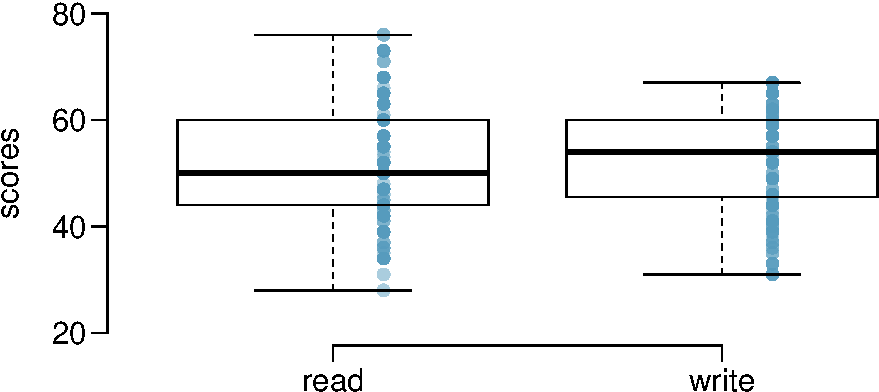
\includegraphics[width=0.5\linewidth]{Homework_7_files/figure-latex/unnamed-chunk-4-1}
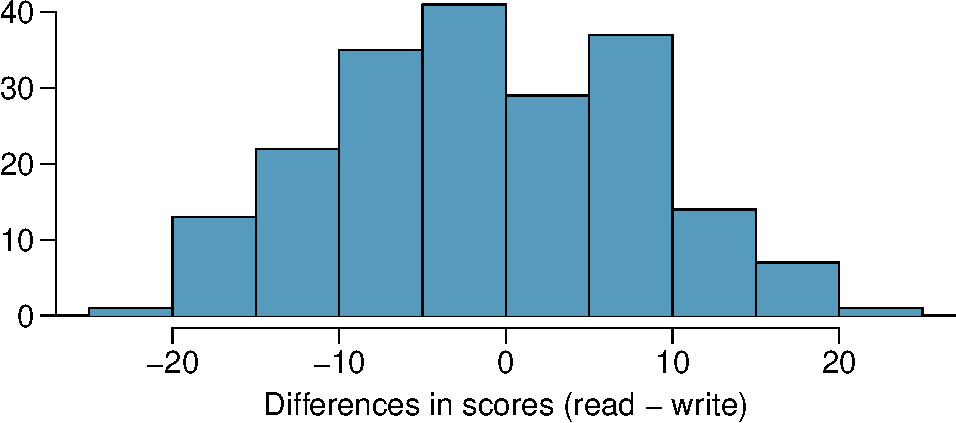
\includegraphics[width=0.5\linewidth]{Homework_7_files/figure-latex/unnamed-chunk-4-2}

\begin{enumerate}
\def\labelenumi{(\alph{enumi})}
\tightlist
\item
  Is there a clear difference in the average reading and writing scores?
\end{enumerate}

\emph{The boxplots shows that there is some difference in reading and
writing scores. The median for the writing appears to be higher. The
75th and 25th percentile line are somewhat close. The maximum for
reading appears to be much higher than maximum score for writing.The
reading - writing histogram show a spread from around -20 to 20. So
there is a difference, but we can't tell if this difference is
significant.}

\begin{enumerate}
\def\labelenumi{(\alph{enumi})}
\setcounter{enumi}{1}
\tightlist
\item
  Are the reading and writing scores of each student independent of each
  other?
\end{enumerate}

\emph{The sample is random and less than 10\% of the total population.
Thus we can assume that the scores of each other are independent}

\begin{enumerate}
\def\labelenumi{(\alph{enumi})}
\setcounter{enumi}{2}
\tightlist
\item
  Create hypotheses appropriate for the following research question: is
  there an evident difference in the average scores of students in the
  reading and writing exam?
\end{enumerate}

\emph{H0: There is no difference in the reading and writting scores}
\emph{HA: There is a difference in the reading and writting scores}

\begin{enumerate}
\def\labelenumi{(\alph{enumi})}
\setcounter{enumi}{3}
\tightlist
\item
  Check the conditions required to complete this test.
\end{enumerate}

\emph{Independence: yes, the scores of each student are independent of
each other.} \emph{Sample size is less than 10\% of the total
population} \emph{Distribution: is a normal distribution}

\begin{enumerate}
\def\labelenumi{(\alph{enumi})}
\setcounter{enumi}{4}
\tightlist
\item
  The average observed difference in scores is
  \({ \widehat { x } }_{ read-write }=-0.545\), and the standard
  deviation of the differences is 8.887 points. Do these data provide
  convincing evidence of a difference between the average scores on the
  two exams?
\end{enumerate}

\begin{Shaded}
\begin{Highlighting}[]
\NormalTok{n <-}\StringTok{ }\DecValTok{200}
\NormalTok{avg_red_wrt <-}\StringTok{ }\FloatTok{-0.545}
\NormalTok{sd_red_wrt <-}\StringTok{ }\FloatTok{8.887}
\NormalTok{SE <-}\StringTok{ }\NormalTok{sd_red_wrt}\OperatorTok{/}\KeywordTok{sqrt}\NormalTok{(n)}
\NormalTok{SE}
\end{Highlighting}
\end{Shaded}

\begin{verbatim}
## [1] 0.6284058
\end{verbatim}

\begin{Shaded}
\begin{Highlighting}[]
\NormalTok{t_score <-}\StringTok{ }\NormalTok{(avg_red_wrt }\OperatorTok{-}\StringTok{ }\DecValTok{0}\NormalTok{)}\OperatorTok{/}\NormalTok{SE}
\NormalTok{t_score}
\end{Highlighting}
\end{Shaded}

\begin{verbatim}
## [1] -0.867274
\end{verbatim}

\begin{Shaded}
\begin{Highlighting}[]
\NormalTok{P_value <-}\StringTok{ }\KeywordTok{pt}\NormalTok{(t_score, n}\DecValTok{-1}\NormalTok{, }\DataTypeTok{lower.tail =} \OtherTok{TRUE}\NormalTok{)}
\KeywordTok{paste0}\NormalTok{(}\StringTok{"The P_value is "}\NormalTok{,P_value)}
\end{Highlighting}
\end{Shaded}

\begin{verbatim}
## [1] "The P_value is 0.193418237099674"
\end{verbatim}

\emph{This is about 0.20 or about 20\% likelihood of seeing an average
difference of -0.545 if the the null hypothesis is true that there is no
difference.This is strong evidence to fail to reject the null
hypothesis.}

\begin{enumerate}
\def\labelenumi{(\alph{enumi})}
\setcounter{enumi}{5}
\tightlist
\item
  What type of error might we have made? Explain what the error means in
  the context of the application.
\end{enumerate}

\emph{If there is a difference, then we would have made a type II error
since we failed to reject the null hypothesis.It means that there is
really a difference in the average scores between reading and writing
and we failed to detect it}

\begin{enumerate}
\def\labelenumi{(\alph{enumi})}
\setcounter{enumi}{6}
\tightlist
\item
  Based on the results of this hypothesis test, would you expect a
  confidence interval for the average difference between the reading and
  writing scores to include 0? Explain your reasoning.
\end{enumerate}

\emph{average difference between the reading and writing scores to
include 0? Explain your reasoning. Based on the findings above, I would
expect the confidence interval to include 0.}

\begin{Shaded}
\begin{Highlighting}[]
\NormalTok{SE <-}\StringTok{ }\NormalTok{sd_red_wrt}\OperatorTok{/}\KeywordTok{sqrt}\NormalTok{(n)}
\NormalTok{t_score <-}\StringTok{ }\KeywordTok{qt}\NormalTok{(}\DataTypeTok{p=}\NormalTok{(}\FloatTok{0.05}\OperatorTok{/}\DecValTok{2}\NormalTok{), n}\DecValTok{-1}\NormalTok{, }\DataTypeTok{lower.tail =} \OtherTok{FALSE}\NormalTok{)}
\NormalTok{t_score}
\end{Highlighting}
\end{Shaded}

\begin{verbatim}
## [1] 1.971957
\end{verbatim}

\begin{Shaded}
\begin{Highlighting}[]
\NormalTok{upper <-}\StringTok{ }\NormalTok{avg_red_wrt }\OperatorTok{+}\StringTok{ }\NormalTok{SE }\OperatorTok{*}\StringTok{ }\NormalTok{t_score}
\NormalTok{lower <-}\StringTok{ }\NormalTok{avg_red_wrt }\OperatorTok{-}\StringTok{ }\NormalTok{SE }\OperatorTok{*}\StringTok{ }\NormalTok{t_score}
\KeywordTok{c}\NormalTok{(upper, lower)}
\end{Highlighting}
\end{Shaded}

\begin{verbatim}
## [1]  0.6941889 -1.7841889
\end{verbatim}

\begin{center}\rule{0.5\linewidth}{\linethickness}\end{center}

\clearpage

\textbf{Fuel efficiency of manual and automatic cars, Part II.} (7.28,
p.~276) The table provides summary statistics on highway fuel economy of
cars manufactured in 2012. Use these statistics to calculate a 98\%
confidence interval for the difference between average highway mileage
of manual and automatic cars, and interpret this interval in the context
of the data.

\begin{tabular}{l c c }
\hline
        & \multicolumn{2}{c}{Hwy MPG} \\
\hline
            & Automatic     & Manual         \\
Mean    & 16.12         & 19.85          \\
SD      & 3.58          & 4.51           \\
n       & 26            & 26 \\
\hline
& \\
& \\
\end{tabular}

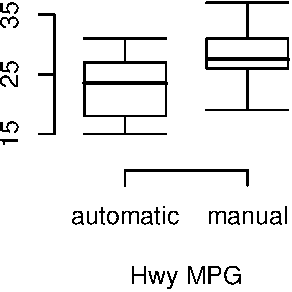
\includegraphics{Homework_7_files/figure-latex/unnamed-chunk-7-1.pdf}

H0: The average miles difference is equal to 0. HA: The average miles
difference is not equal to 0.

\begin{Shaded}
\begin{Highlighting}[]
\NormalTok{n_man <-}\StringTok{ }\DecValTok{26}
\NormalTok{n_auto <-}\StringTok{ }\DecValTok{26}
\NormalTok{mean_auto <-}\StringTok{ }\FloatTok{16.12}
\NormalTok{mean_man <-}\StringTok{ }\FloatTok{19.85}

\NormalTok{sd_auto <-}\StringTok{ }\FloatTok{3.58}
\NormalTok{sd_man <-}\StringTok{ }\FloatTok{4.51}

\NormalTok{diff_mean <-}\StringTok{  }\NormalTok{mean_man }\OperatorTok{-}\StringTok{ }\NormalTok{mean_auto}
\NormalTok{diff_mean}
\end{Highlighting}
\end{Shaded}

\begin{verbatim}
## [1] 3.73
\end{verbatim}

\begin{Shaded}
\begin{Highlighting}[]
\NormalTok{diff_sd <-}\StringTok{ }\NormalTok{sd_man }\OperatorTok{-}\StringTok{ }\NormalTok{sd_auto}
\NormalTok{diff_sd}
\end{Highlighting}
\end{Shaded}

\begin{verbatim}
## [1] 0.93
\end{verbatim}

\begin{Shaded}
\begin{Highlighting}[]
\NormalTok{se <-}\StringTok{ }\KeywordTok{sqrt}\NormalTok{((sd_man}\OperatorTok{^}\DecValTok{2}\OperatorTok{/}\NormalTok{n_man) }\OperatorTok{+}\StringTok{ }\NormalTok{(sd_auto}\OperatorTok{^}\DecValTok{2}\OperatorTok{/}\NormalTok{n_auto))}
\NormalTok{se}
\end{Highlighting}
\end{Shaded}

\begin{verbatim}
## [1] 1.12927
\end{verbatim}

\begin{Shaded}
\begin{Highlighting}[]
\NormalTok{t <-}\StringTok{ }\NormalTok{(diff_mean }\OperatorTok{-}\StringTok{ }\DecValTok{0}\NormalTok{)}\OperatorTok{/}\NormalTok{se}
\NormalTok{t}
\end{Highlighting}
\end{Shaded}

\begin{verbatim}
## [1] 3.30302
\end{verbatim}

\begin{Shaded}
\begin{Highlighting}[]
\NormalTok{p <-}\StringTok{ }\KeywordTok{pt}\NormalTok{(t, n}\DecValTok{-1}\NormalTok{, }\DataTypeTok{lower.tail =} \OtherTok{FALSE}\NormalTok{)}
\NormalTok{p}
\end{Highlighting}
\end{Shaded}

\begin{verbatim}
## [1] 0.0005670179
\end{verbatim}

Since p-value \textless{} 0.05, reject H0. The data provide strong
evidence that the there is a difference in the average miles.

\begin{center}\rule{0.5\linewidth}{\linethickness}\end{center}

\clearpage

\textbf{Email outreach efforts.} (7.34, p.~284) A medical research group
is recruiting people to complete short surveys about their medical
history. For example, one survey asks for information on a person's
family history in regards to cancer. Another survey asks about what
topics were discussed during the person's last visit to a hospital. So
far, as people sign up, they complete an average of just 4 surveys, and
the standard deviation of the number of surveys is about 2.2. The
research group wants to try a new interface that they think will
encourage new enrollees to complete more surveys, where they will
randomize each enrollee to either get the new interface or the current
interface. How many new enrollees do they need for each interface to
detect an effect size of 0.5 surveys per enrollee, if the desired power
level is 80\%?

\[
\begin{aligned}
n=\left( \frac { { Z }_{ 0.05 }+{ Z }_{ 0.8 } }{ estimated\quad size }  \right) ^{ 2 }\times 2SE^{ 2 }
\end{aligned}
\] \[
\begin{aligned}
n=\left( \frac { 1.96+0.84 }{ 0.5 }  \right) ^{ 2 }\times \sqrt { { 2.2 }^{ 2 }+{ 2.2 }^{ 2 } } 
\end{aligned}
\]

\begin{Shaded}
\begin{Highlighting}[]
\CommentTok{# alpha = 0.05, z0.8 = 0.84, z0.05 = 1.96}
\NormalTok{sd <-}\StringTok{ }\FloatTok{2.2}
\NormalTok{es <-}\StringTok{ }\FloatTok{0.5}
\NormalTok{n <-}\StringTok{ }\NormalTok{(((}\FloatTok{0.84} \OperatorTok{+}\StringTok{ }\FloatTok{1.96}\NormalTok{)}\OperatorTok{^}\DecValTok{2}\NormalTok{)}\OperatorTok{/}\NormalTok{(}\FloatTok{0.5}\NormalTok{)}\OperatorTok{^}\DecValTok{2}\NormalTok{)}\OperatorTok{*}\NormalTok{(}\DecValTok{2} \OperatorTok{*}\StringTok{ }\FloatTok{2.2}\OperatorTok{^}\DecValTok{2}\NormalTok{)}

\KeywordTok{paste0}\NormalTok{ (}\StringTok{"Number of desired sample size to the power 80% is: "}\NormalTok{,}\KeywordTok{round}\NormalTok{(n, }\DataTypeTok{digits =} \DecValTok{0}\NormalTok{))}
\end{Highlighting}
\end{Shaded}

\begin{verbatim}
## [1] "Number of desired sample size to the power 80% is: 304"
\end{verbatim}

\emph{We should target 304 survey in order to achieve 80\% power at the
0.05 significance level for this context.} \emph{The standard error
difference of 2.8 × SE is specific to a context where the targeted power
is 80\% and the significance level is alpha = 0.05.}

\begin{center}\rule{0.5\linewidth}{\linethickness}\end{center}

\clearpage

\textbf{Work hours and education.} The General Social Survey collects
data on demographics, education, and work, among many other
characteristics of US residents.47 Using ANOVA, we can consider
educational attainment levels for all 1,172 respondents at once. Below
are the distributions of hours worked by educational attainment and
relevant summary statistics that will be helpful in carrying out this
analysis.

\begin{center}
\begin{tabular}{l  r  r  r  r  r  r}
                & \multicolumn{5}{c}{\textit{Educational attainment}} \\
\cline{2-6}
                & Less than HS  & HS    & Jr Coll   & Bachelor's & Graduate & Total \\
\hline
Mean            & 38.67         & 39.6  & 41.39     & 42.55     & 40.85     & 40.45 \\
SD              & 15.81         & 14.97 & 18.1      & 13.62     & 15.51     & 15.17 \\
n               & 121           & 546   & 97        & 253       & 155       & 1,172 \\
\hline
\end{tabular}
\end{center}

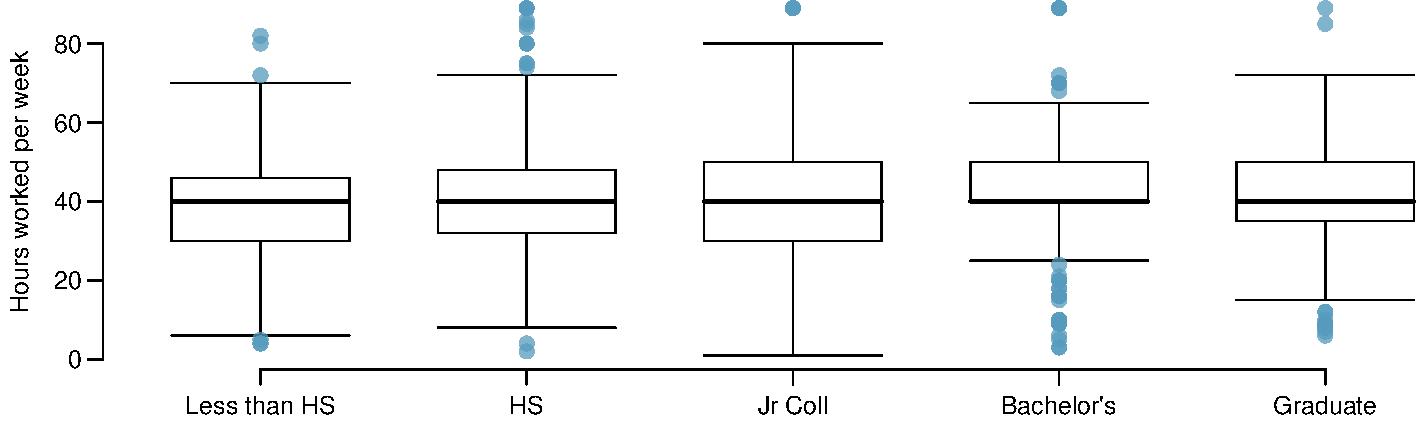
\includegraphics{Homework_7_files/figure-latex/unnamed-chunk-10-1.pdf}

\begin{enumerate}
\def\labelenumi{(\alph{enumi})}
\tightlist
\item
  Write hypotheses for evaluating whether the average number of hours
  worked varies across the five groups.
\end{enumerate}

\emph{H0: The average number of hours worked on all 5 groups are the
same.} \emph{HA: The average number of hours worked on all 5 groups are
\textbf{not} the same}

\begin{enumerate}
\def\labelenumi{(\alph{enumi})}
\setcounter{enumi}{1}
\tightlist
\item
  Check conditions and describe any assumptions you must make to proceed
  with the test.
\end{enumerate}

\emph{Independence: yes, the observation parameters are independent of
each other} \emph{Sample size: the sample size is less than 10\% of the
total population} \emph{The data follows the normal distribution}

\begin{enumerate}
\def\labelenumi{(\alph{enumi})}
\setcounter{enumi}{2}
\tightlist
\item
  Below is part of the output associated with this test. Fill in the
  empty cells.
\end{enumerate}

\begin{center}
\renewcommand{\arraystretch}{1.25}
\begin{tabular}{lrrrrr}
  \hline
            & Df    
                    & Sum Sq        
                            & Mean Sq       
                                    & F-value      
                                            & Pr($>$F) \\ 
  \hline
degree      & \fbox{\textcolor{white}{{\footnotesize XXXXX}}}  
                    & \fbox{\textcolor{white}{{\footnotesize XXXXX}}}       
                            & 501.54    
                                    & \fbox{\textcolor{white}{{\footnotesize XXXXX}}}   
                                            & 0.0682 \\ 
Residuals   & \fbox{\textcolor{white}{{\footnotesize XXXXX}}} 
                    & 267,382     
                            & \fbox{\textcolor{white}{{\footnotesize  XXXXX}}}          
                                    &     
                                            &  \\ 
   \hline
Total       & \fbox{\textcolor{white}{{\footnotesize XXXXX}}} 
                    &\fbox{\textcolor{white}{{\footnotesize XXXXX}}}
\end{tabular}
\end{center}

\begin{Shaded}
\begin{Highlighting}[]
\CommentTok{# we assume that the confidence interval is 95%, alpha is 0.05, p_value = 0.0682 which is > alpha, we fail to reject H0}
\NormalTok{k <-}\StringTok{ }\DecValTok{5} \CommentTok{# number of groups}
\NormalTok{n <-}\StringTok{ }\DecValTok{1172}
\NormalTok{mean_srt <-}\StringTok{ }\FloatTok{501.54}
\NormalTok{sum_srt <-}\StringTok{ }\DecValTok{267382}
\NormalTok{p_value <-}\StringTok{ }\FloatTok{0.0682}

\CommentTok{# get the Df for degree, residential, and total}
\NormalTok{dfg <-}\StringTok{ }\NormalTok{k }\OperatorTok{-}\StringTok{ }\DecValTok{1}
\NormalTok{dfe <-}\StringTok{ }\NormalTok{n }\OperatorTok{-}\StringTok{ }\NormalTok{k}
\NormalTok{dft <-}\StringTok{ }\NormalTok{dfg }\OperatorTok{+}\StringTok{ }\NormalTok{dfe}
\NormalTok{df <-}\StringTok{ }\KeywordTok{c}\NormalTok{(dfg, dfe, dft)}
\NormalTok{df}
\end{Highlighting}
\end{Shaded}

\begin{verbatim}
## [1]    4 1167 1171
\end{verbatim}

\begin{Shaded}
\begin{Highlighting}[]
\CommentTok{# find summation sqrt}
\NormalTok{sumation_rt_degree <-}\StringTok{ }\NormalTok{dfg }\OperatorTok{*}\StringTok{ }\NormalTok{mean_srt}
\NormalTok{sumation_rt_resd <-}\StringTok{ }\NormalTok{sum_srt }\OperatorTok{+}\StringTok{ }\NormalTok{sumation_rt_degree}
\NormalTok{total <-}\StringTok{ }\KeywordTok{c}\NormalTok{(sumation_rt_degree, sum_srt, sumation_rt_resd)}
\NormalTok{total}
\end{Highlighting}
\end{Shaded}

\begin{verbatim}
## [1]   2006.16 267382.00 269388.16
\end{verbatim}

\begin{Shaded}
\begin{Highlighting}[]
\CommentTok{# find mean sqrt }
\NormalTok{mean_res <-}\StringTok{ }\NormalTok{sum_srt }\OperatorTok{/}\StringTok{ }\NormalTok{dfe}
\NormalTok{mean_res}
\end{Highlighting}
\end{Shaded}

\begin{verbatim}
## [1] 229.1191
\end{verbatim}

\begin{Shaded}
\begin{Highlighting}[]
\CommentTok{# find the f-value}
\NormalTok{f_value <-}\StringTok{ }\NormalTok{mean_srt }\OperatorTok{/}\StringTok{ }\NormalTok{mean_res}
\NormalTok{f_value}
\end{Highlighting}
\end{Shaded}

\begin{verbatim}
## [1] 2.188992
\end{verbatim}

\begin{enumerate}
\def\labelenumi{(\alph{enumi})}
\setcounter{enumi}{3}
\tightlist
\item
  What is the conclusion of the test?
\end{enumerate}

\emph{P(\textgreater{}\(F\)): 0.0682 At significance level of 0.05, we
fail to reject the null hypothesis that the means of the groups are
different. There is about a 7\% chance that this kind of variability is
present when the means of the groups are the same.}


\end{document}
